\documentclass[times, utf8, zavrsni]{fer}

\usepackage{booktabs}
\usepackage[hidelinks]{hyperref}
\usepackage{float}

\begin{document}

\thesisnumber{000}
\title{Klasifikacija uporabom umjetnih neuronskih mreža}
\author{Darijo Brčina}

\maketitle

% Ispis stranice s napomenom o umetanju izvornika rada. Uklonite naredbu \izvornik ako želite izbaciti tu stranicu.
\izvornik

% Dodavanje zahvale ili prazne stranice. Ako ne želite dodati zahvalu, naredbu ostavite radi prazne stranice.
\zahvala{}

\tableofcontents

\chapter{Uvod}
Uvod rada. Nakon uvoda dolaze poglavlja u kojima se obrađuje tema.

\chapter{{Pregled područja}}
Pitate li se ikada što je to inteligencija te čemu nam služi. To pitanje postavljeno je još za vrijeme začetka filozofije kao znanosti kada su se tadašnji filozofi pitali kako i na koji način je ljudsko razmišljanje, učenje i pamćenje ostvareno. Ni dan danas ne postoji jednoznačan odgovor na to pitanje jer ljudski mozak i dalje predstavlja jednu veliku nepoznanicu koja vjerojatno nikada ili ne tako skoro neće biti razriješena. No znanost je podosta napredovala i shodno tomu se razvila želja da se ljudska inteligencija pokuša pretočiti u nekakvu vrstu inteligencije strojeva.

Početak ovakvog razmišljanja datira od 50-tih godina dvadesetog stoljeća kada Alan Turing u članku \textit{Computing Machinery and Intelligence} časopisa \textit{Mind} postavlja pitanje: Mogu li strojevi misliti? \engl{Can machines think?} na koje pokušava odgovoriti kroz tzv. igru imitacije \engl{imitation game}. Sudionici igre su tri igrača: igrač A, igrač B i igrač C gdje su igrači A i B ispitanici a igrač C ispitivač. Cilj igrača C je utvrditi spol ispitanika postavljanjem pitanja, cilj igrača B je pomoći ispitivaču C a cilj igrača A je navesti ispitivača C na pogrešnu identifikaciju. Što će se dogoditi ako stroj uzme mjesto igrača A? Ako broj pogrešaka igrača C bude gotovo jednak u oba slučaja, onda je stroj inteligentan. \citep{turingAI}. Ovakav princip se često naziva turingov test \engl{Turing test}.

Nedugo nakon turingovog eksperimenta, 1956. se održava konferencija u Dartmouthu \citep{wiki:DART} na inicijativu John McCarthy-a, tadašnjeg mladog profesora matematike na fakultetu u Dartmouthu, koji okuplja oko sebe nekolicinu znanstvenika i prijatelja kako bi pokušali koncepte ljudske inteligencije preslikati u inteligenciju strojeva. Cilj je pokazati kako strojevi koriste jezik, kako zaključuju i stvaraju apstraktne koncepte i kako vremenom postaju sve prilagodljiviji na predočene probleme baš kao i ljudi. Inicijalna ideja je bila da se neki od navedenih problema može dokazati uz manju skupinu dobrih znanstvenika i kroz period od jednog ljeta (McCarthy et al. 1955). To naravno nije bilo moguće. Time se formalno uvodi pojam \textit{umjetna inteligencija}.

\section{Umjetna inteligencija}
Kao što je anticipirano ranije, umjetna inteligencija \engl{artificial intelligence} je laički rečeno inteligencija strojeva a znanost koja se jednim dijelom bavi proučavanjem umjetne inteligencije jest računarska znanost \engl{computer science}.

Primjena umjetne inteligencije danas je izrazito rasprostranjena kroz gotovo svaku industriju. Pronalazimo ju u medicini, automobilskoj industriji, robotici, pa i u sportskoj i industriji igara. Jedan od poznatijih događaja koji prikazuje primjenu umjetne inteligencije dogodio se 2016. kada je računalo naziva \textit{AlphaGo} u igri \textit{Go} uspijelo pobijediti svjetskog prvaka Lee Sedolu rezultatom 4:1 te time ostvario velik uspjeh u svijetu umjetne inteligencije kao i pažnju javnosti \citep{moyerGO}.

Umjetnu inteligenciju je dakako potrebno trenirati i učiti pa je tako učenje podijeljeno na dvije veće cjeline:
\begin{center}
    \begin{enumerate}
        \item simboličko učenje te
        \item strojno učenje.
    \end{enumerate}
\end{center}

\subsection{Simboličko učenje}
Simbolička umjetna inteligencija \engl{symbolic artificial intelligence} je izraz koji definira skup istraživačkih metoda koje se temelje na ljudima lako čitljivim simbolima \engl{human-readable simbol} koji modeliraju probleme i logiku. Jedan od najboljih primjera jesu \textit{ekspertni sustavi} koji se temelje na skupu pravila. Pravila su modelirana na sličan način kao i Ako-Onda rečenica \engl{If-Then statement} koja je u ljudskoj komunikaciji svakodnevno u upotrebi. Također, razne vrste logika poput propozicijska \engl{Propositional logic}, često referirana kao Boolova algebra, logika prvog reda \engl{First order logic}, poznatija kao predikatna logika \engl{Predicate logic}, neizrazita logika \engl{Fuzzy logic} pripadaju upravo simboličkoj umjetnoj inteligenciji. Ovakav način učenja bio je popularan početkom 1950. sve do kraja 1980 \citep{wiki:SIMB}.

\subsection{Strojno učenje}
Strojno učenje \engl{machine learning, ML} predstavlja niz metoda i algoritama koji sustavima pružaju stjecanje novog znanja kroz modeliranje obrazaca koje onda kasnije mogu iskoristiti za predviđanje novih podataka ili sličnih \citep{cupicML}. Glavna ideja je da sustavi uče iz iskustva, empirijski, bez da se programska implementacija mijenja što znatno olakšava manipulaciju istih.

Danas postoji nezgrapno puno podataka koje je moguće i koje je potrebno iskoristiti za učenje pa je cilj konstruirati sustave koji mogu iskoristiti baš te podatke za neka korisna ponašanja poput predviđanja i raspoznavanja raznih uzoraka \citep{cupicML}. Podatci se svrstavaju u dvije grupe: \textit{numerički} i \textit{kategorički} podatci. Numerički podatci su svi oni podatci nad kojima je moguće izvršiti aritmetičke operacije. Npr. unos dnevnih kalorija, broj slobodnih bacanja na košarkaškoj utakmici, isplata plaća i sl. Kategorički podatci se dodatno dijele u dvije podgrupe: nominalni i ordinalni podatci. Nominalni podatci su imenovani podatci koji nisu numerički, tj. podatci nad kojima nisu definirane aritmetičke operacije. Npr. podatci o spolu jedinke, osjećaju raspoloženja poput "tužan" ili "veseo" i sl. Ordinalni podatci također nemaju definiranu aritmetiku, no imaju definiran prirodan poredak i mogu se uspoređivati. Npr. mišljenje jedne osobe može biti "jako zadovoljan" dok druge "zadovoljan" što možemo usporediti i konstruirati prirodan poredak.

Strojno učenje dijelimo na četiri područja:
\begin{center}
    \begin{enumerate}
        \item nadzirano učenje,
        \item nenadzirano učenje,
        \item polu-nadzirano učenje te
        \item podržano učenje.
    \end{enumerate}
\end{center}

\textit{Nadzirano učenje} je tema ovog rada pa će biti obrađeno detaljnije u narednom poglavlju.

\bigskip

\textit{Nenadzirano učenje} \engl{unsupervised learning} je vrsta učenja u kojem skup podataka predstavljaju samo ulazni podatci bez znanja o tome kako bi isti trebali biti tabelirani. Zbog ovakvog pristupa, učenje je i dobilo ime nenadzirano učenje, tj. učenje bez prisustva učitelja \engl{supervisor}. Najpoznatiji postupak nenadzirano učenja je postupak grupiranja \engl{clustering}. Cilj grupiranja je na temelju danih podataka pokušati pronaći sve podatke koji imaju slična svojstva te ih zatim grupirati u odvojene razrede. Npr. neka skup ulaznih podataka sustava bude mješavina slika ljudi i slika automobila. Kao konačni rezultat, moraju se stvoriti dva razreda: razred ljudi te razred automobila. Na slici \ref{fig:clustering} prikazan je primjer grupiranja.

\begin{figure}[H]
    \centering
    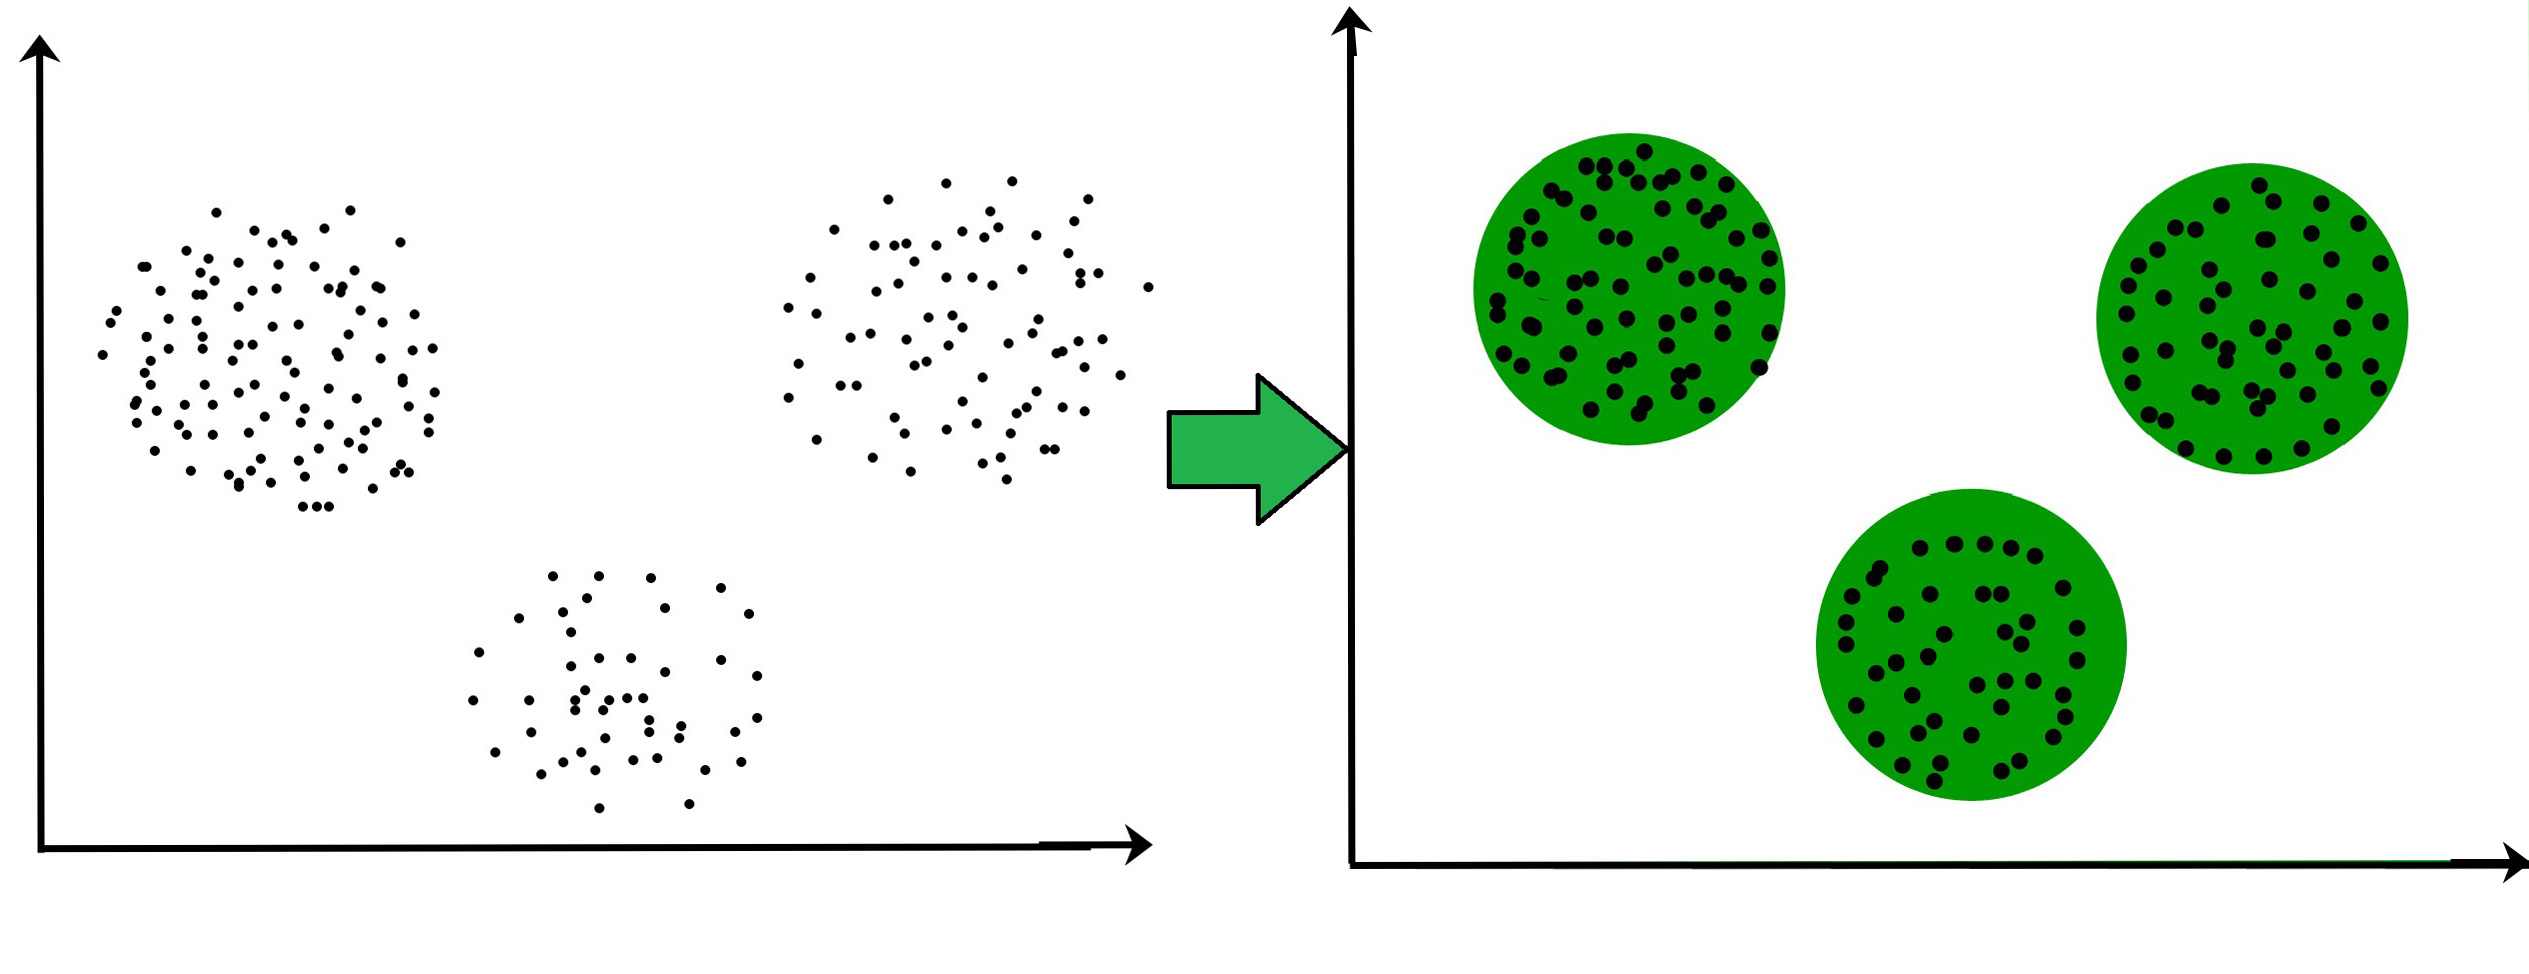
\includegraphics[scale=0.75]{img/clustering.jpg}
    \caption[Caption for LOF]{Primjer grupiranja\footnotemark}
    \label{fig:clustering}
\end{figure}
\footnotetext{Preuzeto sa https://www.geeksforgeeks.org/clustering-in-machine-learning/.}

Uz grupiranje poznati postupci su i postupci smanjenja dimenzionalnosti \engl{dimensionality reduction}, postupci otkrivanja stršećih ili novih vrijednosti \engl{outlier detection, novelty detection} i drugi.

\bigskip

\textit{Polu-nadzirano učenje} \engl{semi-supervised learning}, kao što samo ime nalaže, je učenje u kojem se isprepliću koncepti nadzirano učenje sa konceptima nenadziranim učenjem. Ono pokazuje dosta veće uspjehe nego navedeni, izvedba je izrazito zahtjevnija \citep{wiki:SEMISUP}.

\bigskip

\textit{Podržano učenje} \engl{reinforcement learning, RL} je vrsta učenja koja se potpuno razlikuje od svih do sada navedenih jer ono ne očekuje nikakve tabelirane ulazne ili izlazne podatke već je glavna ideja optimizacija ponašanja računalnih agenata. Razmatra se interakcija agenta sa okolinom \engl{environment} kroz niz akcija za koje isti može biti nagrađen ili kažnjen ovisno o ishodu akcije. Željeni cilj agenta je maksimizirati mogući dobitak nagrade \citep{wiki:RL}. Na slici \ref{fig:reinforcement-learning} prikazan je model podržanog učenja.

\begin{figure}[H]
    \centering
    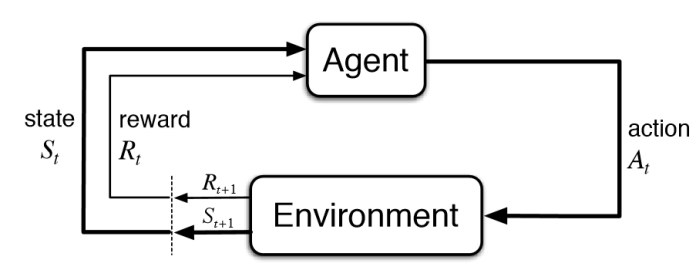
\includegraphics[scale=0.7]{img/reinforcement-learning.jpg}
    \caption[Caption for LOF]{Model podržanog učenja\footnotemark}
    \label{fig:reinforcement-learning}
\end{figure}
\footnotetext{Preuzeto sa https://www.kdnuggets.com/2018/03/5-things-reinforcement-learning.html/.}

\chapter{Nadzirano učenje}
Nadzirano učenje \engl{supervised learning} je vrsta učenja čiji je cilj sve podatke koji dođu na ulaz sustava preslikati u izlaz koji točno odgovara predanim ulazima. Dakle, prije samog učenja poznati su ulazi, koji se često modeliraju vektorima, te izlazi, koji su pridruženi tim ulazima i predstavljaju jedan podatak, stoga se tijekom učenja u svakom trenutku zna željeni izlaz te se za krive rezultate daje određena povratna informacija \engl{feedback} o tome koliko sustav griješi. Upravo zbog navedenog koncepta je učenje i dobilo ime nadzirano učenje jer se proces učenja izvršava uz prisustvo učitelja \engl{supervisor}. Razlikujemo dvije faze strojnog modela prikazane na slici \ref{fig:supervised-learning-flow}:
\begin{enumerate}
    \item faza učenja modela te
    \item faza iskorištavanja modela.
\end{enumerate}

\section{Učenje modela}

\begin{figure}[H]
    \centering
    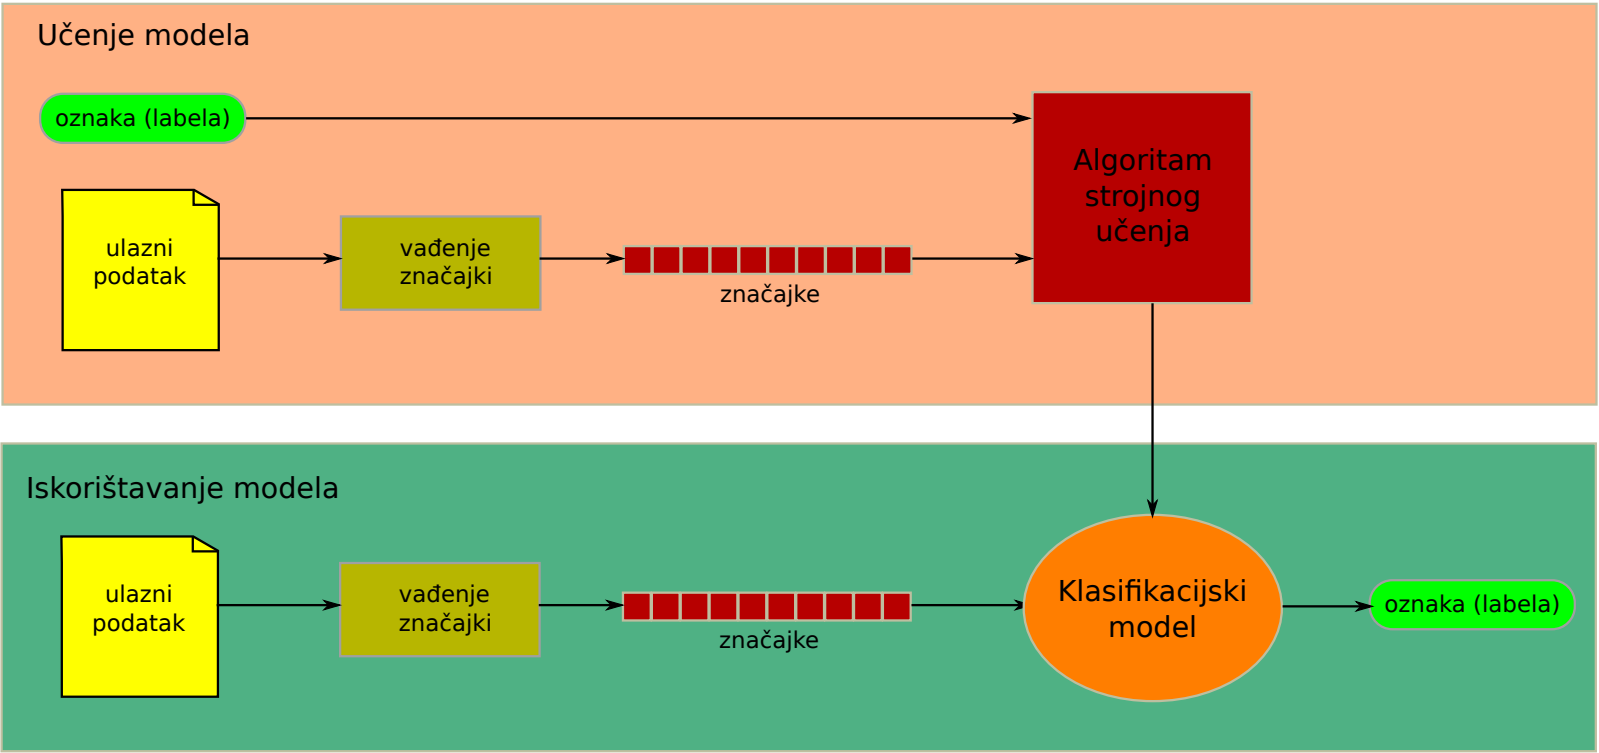
\includegraphics[scale=0.5]{img/supervised-learning-flow.png}
    \caption[Caption for LOF]{Model strojnog učenja\footnotemark}
    \label{fig:supervised-learning-flow}
\end{figure}
\footnotetext{Preuzeto iz literature \citep{cupicML}.}

Tijekom faze učenja, modelu se predaje skup ulaznih podataka za učenje \engl{training set}. Svaki podatak skupa možemo notirati kao $(\textbf{x}, y)\textsubscript{i}$ što predstavlja \textit{i}-ti primjer iz skupa za učenje gdje \textbf{x} predstavlja vektor ulaznih podataka, a \textit{y} vrijednost pridružena ulaznom vektoru, odnosno oznaku \engl{label}. Ulazni podatak često može biti kompleksne naravi što znači da ga je potrebno "razbiti" u manje cjeline. Takav postupak se naziva vađenje značajki \engl{feature extraction}. Rezultat navedenog je kolekcija značajki koja se zatim predaje određenom algoritmu strojnog učenja. Npr. ulazni podatci mogu biti razne gume poput gume automobila, gume bicikla, gume traktora i sl. a značajka bi onda mogla biti volumen gume, oblik gume, boja gume i sl. Algoritam strojnog učenja će na temelju predanih značajki pokušati optimizirati parametre odabranog modela kako bi se isti mogao koristiti u sljedećoj fazi.

\bigskip

Faza iskorištavanja modela predstavlja fazu u kojoj se treba utvrditi radi li naučeni model sa podatcima nad kojima nije učio, tj. je li razvio sposobnost generalizacije \engl{generalization}. Ako model dodijeli točnu oznaku za većinu ulaznih podataka, onda možemo reći da je razvio svojstvo generalizacije. No što ako u velikoj mjeri ne uspije točno povezati izlaze sa ulazima? Ako dođe to takve pojave, kažemo da je model pretreniran \engl{overfitting}. Do navedene pojave dolazi kada model nauči previše nad skupom podataka za učenje, tj. podatke za učenje nauči savršeno raspoznavati dok za nove podatke ne uspijeva dati željene rezultate. Postoji nekoliko načina kako se može utjecati da model razvije svojstvo generalizacije a spomenut ćemo samo jedan od njih, \textit{unakrsna provjera}.

\bigskip

Unakrsna provjera \engl{cross-validation} je postupak koji se koristi tijekom faze učenja modela. Ideja je da se dio podataka iz skupa za učenje razdijeli u novi skup, skup za provjeru \engl{validation set}. Skup za provjeru često sadrži od 20\% do 30\% svih podataka iz skupa za učenje \citep{cupicML}. Tijekom faze učenja modela, model će i dalje učiti samo nad skupom za učenje dok ćemo mu povremeno dati i podatke iz skupa za provjeru čisto da se vidi koliko griješi nad njima. Važno je napomenuti da model nad podatcima iz skupa za provjeru neće učiti, tj. neće optimizirati parametre već će bit prisiljen da nauči generalizirati. Postavlja se pitanje do kada će faza učenja modela onda trajati i odgovor je vrlo jasan. Trajat će do trenutka kada pogreška nad skupom za provjeru počinje rasti. Dijagram na slici \ref{fig:cross-validation} prikazuje kako model uči kroz epohe\footnote{Epoha je ništa drugo nego jedna iteracija učenja, ali u strojnom učenju se često koristi izraz epoha pa ćemo se držati konvencije.}.

\begin{figure}[H]
    \centering
    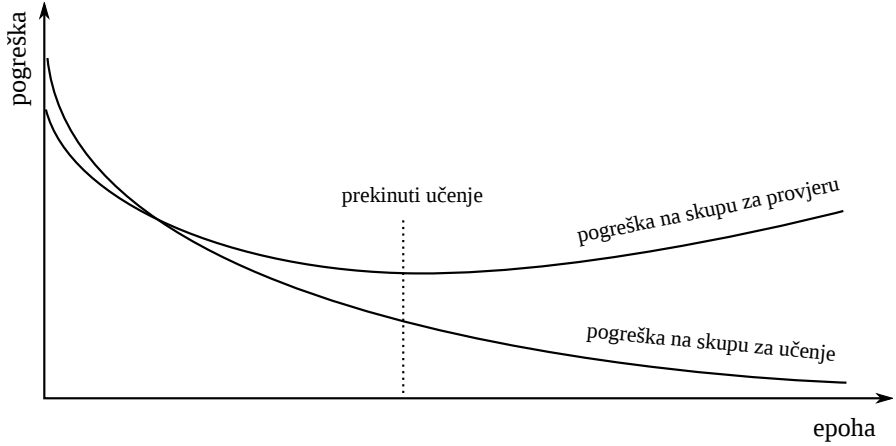
\includegraphics[scale=0.5]{img/cross-validation.png}
    \caption[Caption for LOF]{Kretanje pogrešaka pri učenju strojnog modela\footnotemark}
    \label{fig:cross-validation}
\end{figure}
\footnotetext{Preuzeto iz literature \citep{cupicANN}.}

Također postoji mogućnost da neki od parametara modela utječu na njegovu složenost. Shodno tomu se uvodi još jedan skup, skup za testiranje \engl{testing set}. Ideja je sljedeća: skup podataka razdijelimo u sva tri do sada navedena skupa i normalno provedemo fazu učenja modela uz malu promjenu. Umjesto da se zadovoljimo samo jednim naučenim modelom, pokušavamo pronaći onaj model koji će najbolje minimizirati pogrešku nad skupom za testiranje \citep{cupicML}.

\section{Problemi nadziranog učenja}

Zadatak nadziranog učenja je sljedeći: pretpostavimo da imamo skup za učenje koji se sastoji od \textit{N} različitih parova ulaza i izlaza;
\[(\textbf{x}\textsubscript{1}, y\textsubscript{1}), (\textbf{x}\textsubscript{2}, y\textsubscript{2}),
(\textbf{x}\textsubscript{3}, y\textsubscript{3}),...,
(\textbf{x}\textsubscript{N}, y\textsubscript{N})\]
gdje \textbf{x\textsubscript{i}} predstavlja \textit{i}-ti vektor ulaznih podataka dok \textit{y\textsubscript{i}} \textit{i}-ti željeni izlaz koji je generiran nekom nepoznatom funkcijom $y=f(x)$. \newline
Potrebno je pronaći takvu funkciju \textit{h} koja će najbolje aproksimirati funkciju \textit{f}.

Funckija \textit{h} naziva se hipoteza \engl{hypothesis} i pripada nekom skupu svih hipoteza \textbf{H} koje donekle aproksimiraju zadanu funkciju \textit{f}, neke bolje, neke lošije. U ovom trenutku uključujemo skup za testiranje u proces učenja jer je potrebno pronaći onu hipotezu za koju će aproksimacija biti najbolja, tj. ukupna pogreška generirana tijekom učenja modela bit će minimalna. Time će se osigurati da model poprimi svojstvo generalizacije. Često se pokazuje da je funkcija \textit{f} stohastička \engl{stochastic}, što znači da ne ovisi uvijek samo o varijabli \textit{x} pa se mora koristiti i uvjetovana vjerojatnost $P(Y|x)$ tijekom faze učenja modela \citep{russelAI}\footnote{Iz poglavlja 18.2 Supervised learning.}.

Kao što je rečeno ranije, \textit{y\textsubscript{i}} predstavlja \textit{i}-ti željeni izlaz za \textit{i}-ti ulaz te može poprimiti vrijednost broja ili vrijednost iz nekog konačnog skupa podataka. Ako je slučaj da je izlaz broj, radi se o problemu koji se naziva \textit{regresija}, a ako je slučaj da je izlaz vrijednost iz nekog konačnog skupa podataka, onda se radi o problemu koji se naziva \textit{klasifikacija}.

\subsection{Regresija}
Regresija \engl{regression} je tehnika, tj. algoritam nadziranog učenja koji se koristi kada je potrebno predvidjeti određeni iznos neke funkcije u odnosu na određene parametre. Dakle, dane podatke potrebno je aproksimirati nekom proizvoljnom funkcijom \textit{h} koja je često polinomijalna. Postoje različite vrste regresije pa spomenimo neke od njih. 

Prije svega, postoji regresija s jednom varijablom \engl{regression with one variable} i regresija sa više varijabli \engl{multivariate regression}. Razlika je očita, no pokažimo to na kratkom primjeru. Recimo da želimo modelirati cijene obiteljskih kuća u okolici Zagreba. Za to su nam potrebni neki parametri na temelju kojih ćemo moći vršiti predikcije kao npr. broj kvadratnih metara (m\textsuperscript{2}), broj spavaćih soba, blizina vrtića i škola, povezanost sa javnim prijevozom i sl. U slučaju regresije s jednom varijablom, za modeliranje bi uzeli samo jedan od navedenih parametara, dok bi u slučaju regresije sa više varijabli uzeli sve ili dio navedenih. Dakle, očigledno je da je regresija s jednom varijablom konkretan slučaj regresije sa više varijabli.

\bigskip

\textit{Linearna regresija} \engl{linear regression} je tip regresije koji koristi linearnu krivulju (pravac), tj. polinom prvog stupnja kao aproksimacijsku krivulju.

\textit{Polinomijalna regresija} \engl{polynom regression} je tip regresije koji koristi polinom reda \textit{r} kao aproksimacijsku krivulju.

Na slikama \ref{fig:linear-regression} i \ref{fig:polynom-regression} su prikazani navedeni tipovi regresija.

\bigskip

Dakle, regresija je metoda koja se koristi za predviđanje numeričkih ishoda.

\begin{figure}[H]
    \centering
    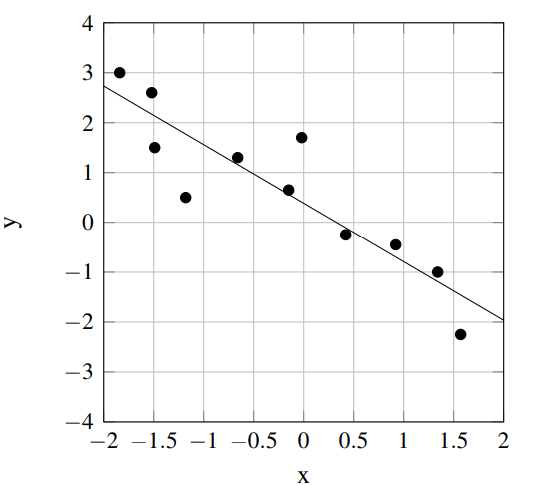
\includegraphics[scale=0.75]{img/linear-regression.png}
    \caption[Caption for LOF]{Primjer linearne regresije\footnotemark}
    \label{fig:linear-regression}
\end{figure}
\footnotetext{Preuzeto iz literature \citep{cupicML}.}

\begin{figure}[H]
    \centering
    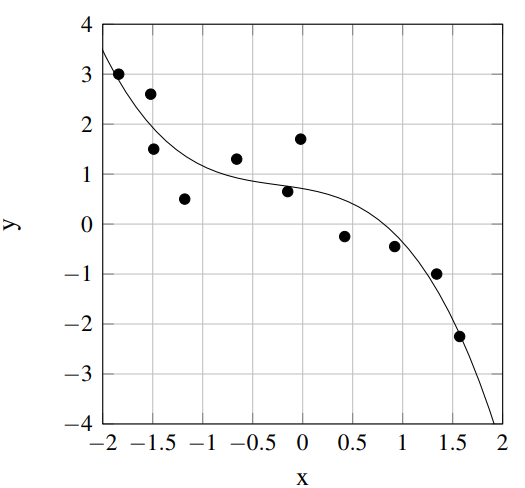
\includegraphics[scale=0.75]{img/polynom-regression.png}
    \caption[Caption for LOF]{Primjer polinomijalne regresije sa kubnim polinomom\footnotemark}
    \label{fig:polynom-regression}
\end{figure}
\footnotetext{Preuzeto iz literature \citep{cupicML}.}

\subsection{Klasifikacija}
Klasifikacija \engl{classification} je tehnika, tj. algoritam nadziranog učenja koji se koristi kada je određeni ulazni podatak potrebno smjestiti odnosno klasificirati kao pripadnika određenog razreda. Izlazi tako organiziranog modela često poprimaju diskretne vrijednosti za razliku od regresije i takav model onda nazivamo klasifikator \engl{classifier}. Razlikujemo nekoliko različitih tipova klasifikatora:

\begin{enumerate}
    \item binarni klasifikator,
    \item višerazredni klasifikator te
    \item klasifikator više oznaka.
\end{enumerate}

\smallskip

Binarni klasifikator \engl{binary classifier} je tip klasifikatora koji zna odrediti pripada li ulazni podatak jednom od ukupno dva moguća razreda. Npr. sustav kao ulaze prima slike na kojima se nalazi ili mačka ili pas. Jednom naučeni klasifikator bi na temelju predane slike morao moći odrediti što se nalazi na slici, mačka ili pas. Naravno uz uvjet da se preda slika mačke ili psa.

Višerazredni klasifikator \engl{multi-class classifier} je tip klasifikatora koji zna odrediti pripada li ulazni podatak jednom od barem tri moguća razreda. Dakle, mora postojati minimalno tri različita razreda kako bi se klasifikator nazivao višerazrednim. U ovom radu ćemo se više fokusirati upravo na navedenom klasifikator koji će naučiti raspoznati tri moguća razreda, no o tome nešto kasnije.

Klasifikator više oznaka \engl{multi-label classifier} je tip klasifikatora koji predstavlja generalizaciju višerazrednog klasifikatora. Pogledajmo sljedeći primjer klasifikacije filmova za bolje razumijevanje. Pretpostavimo da film može imati sljedeće oznake: $(12+)$, $(16+)$ i $(18+)$ gdje svaka oznaka predstavlja minimalan broj godina kojih gledaoc filma mora imati. Određivanje oznake za pojedini film je rezultat korištenja višerazrednog klasifikatora jer je potrebno odrediti pripada li film samo jednom od navedene tri oznake. No što ako film poželimo klasificirati pomoću žanrova? Tada nam višerazredni klasifikator neće puno pomoći jer jedan film može imati više oznaka kao npr. "drama" i "komedija" i sl. Tada ćemo koristiti klasifikator više oznaka.

\bigskip

Klasifikaciju, kao i regresiju, možemo podijeliti na \textit{linearnu klasifikaciju} i \textit{nelinearnu klasifikaciju}, odnosno polinomijalnu.

Linearna klasifikacija \engl{linear classification} je tip klasifikacije u kojoj se granica između razreda aproksimira pomoću linearna krivulje, tj. pravca.

Nelinearna klasifikacija \engl{non-linear classification} je tip klasifikacije u kojoj se granica između razreda aproksimira pomoću nelinearne krivulje koja je često polinomijalna.

Ono što je zajedničko u oba slučaja je postojanje granice između razreda koja se u literaturi naziva \textit{decizijska granica} \citep{cupicANN}. O oblicima decizijskih granica će biti riječ kasnije.

Na slikama \ref{fig:linear-classification} i \ref{fig:non-linear-classification} su prikazani primjeri klasifikacija.

\begin{figure}[H]
    \centering
    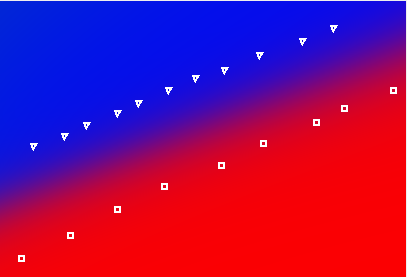
\includegraphics[scale=0.8]{img/linear-classification.png}
    \caption[Caption for LOF]{Primjer linearne klasifikacije\footnotemark}
    \label{fig:linear-classification}
\end{figure}
\footnotetext{Rezultat programske implementacije.}

\begin{figure}[H]
    \centering
    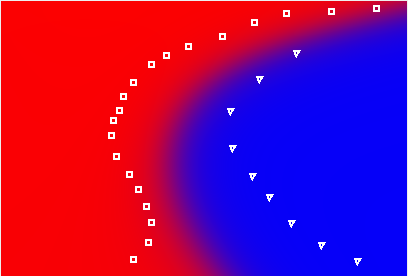
\includegraphics[scale=0.8]{img/non-linear-classification.png}
    \caption[Caption for LOF]{Primjer nelinearne klasifikacije\footnotemark}
    \label{fig:non-linear-classification}
\end{figure}
\footnotetext{Rezultat programske implementacije.}

\section{Algoritmi}
U području nadziranog učenja postoji veliki broj algoritama koji uvelike pridonose boljem učenju. Neki od poznatijih su:

\begin{itemize}
    \item Stroj za podršku vektorima \engl{support-vector machine, SVM},
    \item Stabla odluke \engl{decision trees},
    \item Naivni Bayesov klasifikator \engl{naive Bayes classifier},
    \item Slučajne šume \engl{random forests},
    \item Algoritam k-najbližih susjeda \engl{k-nearest neighbors algorithm},
    \item Umjetna neuronska mreža \engl{artificial neural network} i mnogi drugi.
\end{itemize}

\bigskip

Vidimo da postoji jako velika paleta algoritama od kojih su neki složeniji od drugih, neki daju bolje rezultate od drugih, no niti jedan od algoritama
nije u stanju uvijek dati najbolje rezultate za proizvoljan problem nadziranog učenja \citep{wiki:SUP}. Zbog navedenog vrijedi tzv. \textit{No free lunch} teorem koji nalaže da je za probleme koji zahtijevaju mnogo računalnih resursa poput pretraživanja prostora stanja i optimizacije parametara složenost u prosjeku jednaka za sve metode \citep{wiki:NFL}.

\bigskip
\bigskip

U sljedećem poglavlju ćemo se detaljnije baviti algoritmom \textit{umjetna neuronska mreža}. Pogledat ćemo kako je nastao koncept umjetnog neurona, strukturu umjetnog neurona, arhitekturu unaprijedne neuronske mreže te algoritam kojim unaprijedna neuronska mreža uči.

\chapter{Umjetne neuronske mreže}
U drugom poglavlju (\textit{Pregled područja}) dotaknuli smo se razlika između simboličke umjetne inteligencije i strojnog učenja i rekli smo kako simbolička umjetna inteligencija koristi simbolički pristup, tj. sve iskaze pokušava predočiti u mnoštvo pravila pomoću ljudima čitljivim simbolima, dok se strojno učenje bavi raznim algoritmima pomoću kojih se računalni sustav uči. U ovom poglavlju bavit ćemo se algoritmom strojnog učenja koji koristi tzv. konektivistički pristup.

\section{Motivacija}
Ideja za konektivizmom \engl{connectivism} potaknuta je na temelju strukture ljudskog mozga te zbog izrazite brzine kojom mozak obrađuje podražaje. Danas je poznato da u ljudskom mozgu postoji oko 10\textsuperscript{11} neurona te 10\textsuperscript{15} međusobnih veza što znači da je svaki neuron u prosjeku povezan sa 10\textsuperscript{4} različitih veza \citep{cupicNENR}. To upravo dokazuje da mozak predstavlja jedan kompleksan i paralelan sustav zbog čega je konektivizam dobio ime te čemu algoritam umjetne neuronske mreže teži. Također, koncept ljudskog mozga nije uzet samo radi svoje izrazite brzine prilikom obrade podražaja, već i zbog činjenice da ga se može učiti na temelju velikog broja podataka koji su često ispunjeni raznim šumovima, što je realna situacija, te ga time potaknuti da razvije svojstvo generalizacije. Područje koje se bavi proučavanjem umjetnih neuronskih mreža naziva se neuro-računarstvo \engl{neuro-computing} koje je jedno od grana mekog računarstva \engl{soft-computing}.

\section{Biološki neuron}
Neuroni \engl{neurons} su glavne stanice mozga i živčanog sustava. Zadaća im je da primaju podražaje iz okoline, da prenose određene akcije od mozga prema našim mišićima i da vode računa o pretvaranju električnog potencijala između pojedinih neurona u svim koracima procesa vođenja. Neuron je izgrađen od posebne strukture koja se sastoji od: \textit{tijela stanice} (ili češće \textit{soma}), \textit{dendrita}, \textit{aksona}, i \textit{sinapse}. Struktura biološkog neurona prikazana je na slici \ref{fig:bio-neuron}.

\begin{figure}[H]
    \centering
    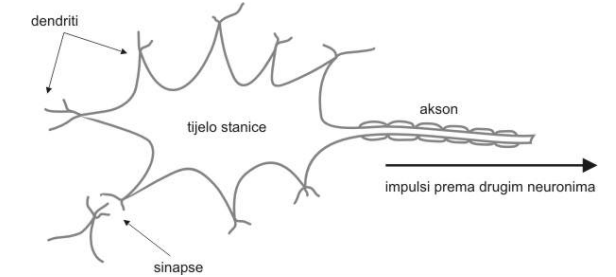
\includegraphics[scale=0.75]{img/bio-neuron.png}
    \caption[Caption for LOF]{Biološki neuron\footnotemark}
    \label{fig:bio-neuron}
\end{figure}
\footnotetext{Preuzeto iz literature \citep{cupicANN}.}

Dendriti \engl{dendrites} su ulazni dijelovi neurona, tj. strukture koje prihvaćaju inpulse od drugih neurona preko veza koje se nazivaju sinapse. Suma svih ulaznih impulsa, tj. potencijala određuje hoće li dotični neuron biti aktiviran ili ne.

Aksoni \engl{axons} su izlazni dijelovi neurona, tj. strukture u kojima se generira određeni električni potencijal koji se dalje prosljeđuje sljedećem neuronu preko sinoptičkih veza.

Sinapse \engl{synapses} su, kao što je rečeno ranije, veze između dendrita jednog neurona i aksona drugog neurona \citep{bioNeuron}.

\section{Umjetni neuron}

\subsection{Povijesni pregled}

\subsubsection{MCP neuron}

\textbf{1943}. dva znanstvenika, Warren S. McCulloch i Walter H. Pitts, u svojem radu \textit{A Logical Calculus of Ideas Immanent in Nervous Activity} definiraju strukturu prvog umjetnog neurona koji se u literaturi često naziva kao \textit{MCP} neuron. Na slici \ref{fig:first-ai-neuron} prikazana je struktura MCP neurona. Dendriti su predstavljeni ulazima označenih slovima \textbf{E} od riječi ekscitacijski\footnote{ekscitacija - uzbuđenje ili aktivirano stanje zbog određenog podražaja (ekscitacija. Hrvatska enciklopedija, mrežno izdanje. Leksikografski zavod Miroslav Krleža, 2020. Pristupljeno 13. 5. 2020. <http://www.enciklopedija.hr/Natuknica.aspx?ID=17398>).} \engl{excitatory} te \textbf{I} od riječi inhibicijski\footnote{inhibicija - kočenje prijenosa živčanih impulsa (inhibicija. Hrvatska enciklopedija, mrežno izdanje. Leksikografski zavod Miroslav Krleža, 2020. Pristupljeno 13. 5. 2020. <http://www.enciklopedija.hr/Natuknica.aspx?ID=27450>).} \engl{inhibitory}, tijelo stanice je predstavljeno slovom \textbf{T} od riječi prag \engl{treshold} dok je akson predstavljen izlazom koji je označen slovom \textbf{Y} bez posebnog značenja.

Ekscitacijski ulazi uzrokuju da neuron postavne aktivan, tj. da se neuron "pali" \engl{fire}, dok inhibicijski ulazi uzrokuju da neuron postane neaktivan, tj. da se neuron "ne pali". Točnije, ako postoji barem jedan inhibicijski ulaz koji je aktivan, tada će neuron sigurno biti neaktivan neovisno o svim ostalim ulazima. Također, ako niti jedan od inhibicijskih ulaza nije aktivan, onda će neuron postati aktivan samo u slučaju kada je suma svih ekscitacijskih ulaza veća ili jednaka pragu, T \citep{McCullPits}. Matematički rečeno \citep{picton2000}:
\begin{equation}
\label{mcp:eq}
    Y = 
    \begin{cases}
        1, & \text{$\sum\limits_{i=1}^n I\textsubscript{i} = 0$ i $\sum\limits_{j=1}^m E\textsubscript{j} \geq T$} \\
        0, & \text{inače.}
    \end{cases}
\end{equation}

\begin{figure}[H]
    \centering
    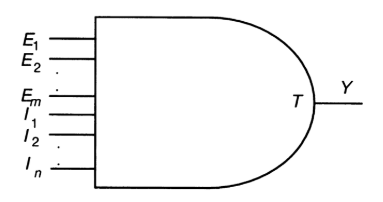
\includegraphics{img/first-ai-neuron.png}
    \caption[Caption for LOF]{MCP neuron\footnotemark}
    \label{fig:first-ai-neuron}
\end{figure}
\footnotetext{Preuzeto iz literature \citep{picton2000} iz poglavlje 1.4.2 Biologically inspired neural networks.}

MCP neuron mogao je modelirati osnovne Booleove logičke operacije kao što su operacija \textit{i} \engl{and}, operacija \textit{ili} \engl{or} i operacija negacije \engl{not} pa se može reći da neuron predstavlja logička vrata \engl{logic gate} što je često korištena struktura prilikom konstrukcija uređaja poput računala koji mogu rješavati kompleksne logičke izraze. Shodno tomu se razvilo vjerovanje da se ljudski mozak sastoji upravo od mnoštva logičkih vrata, no nisu uzimali u obzir činjenicu da takva konstrukcija ne može biti učena te da nema svojstvo generalizacije \citep{picton2000}. 

Postoji još jedna bitna stavka oko strukture MCP neurona koja je prešutno korištena, a to su vrijednosti koje poprimaju ulazi i izlaz. Vrijednosti koje mogu poprimiti su iz skupa $\{0, 1\}$ i niti jedne druge, dok vrijednost praga može biti realan broj. To se implicitno moglo zaključiti iz spomenutih primjena na Boolove logičke operacije te iz formule \eqref{mcp:eq}.

\subsubsection{ADALINE}
\textbf{1960.} dva znanstvenika, Bernard Widrow i Marcian E. Hoff, u svojem radu \textit{Adaptive Switching Circuits} na temelju MCP neurona definiraju jednu od prvih neuronskih mreža nazvanu \textit{ADALINE} \engl{ADAptive LINear Elements}. Na slici \ref{fig:adaline-neuron} prikazana je struktura jednog neurona iz neuronske mreže ADALINE. Dendriti su predstavljeni ulazima označenim slovom \textbf{x}, tijelo stanice predstavljeno je težinama označenim slovom \textbf{w}, a akson je predstavljen izlazom označenim slovom \textbf{y}. Dakle, uočljivo je da postoje neke novine za razliku od MCP neurona. Ulogu ekscitacijskih odnosno inhibicijskih ulaza sada imaju težine koje poprimaju vrijednosti iz realnog skupa brojeva, ulazi i izlaz poprimaju vrijednosti iz skupa $\{-1, 1\}$ i niti jedne druge, osim za ulaz \textbf{x\textsubscript{0}} čija je vrijednost uvijek 1, dok prag više nije eksplicitno zadan, već se u definiciju implicitno uključuje simbolom \textbf{w\textsubscript{0}} koji predstavlja konstantan pomak \engl{bias} \citep{picton2000}.

\begin{figure}[H]
    \centering
    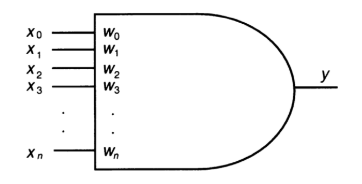
\includegraphics{img/adaline-neuron.png}
    \caption[Caption for LOF]{ADALINE neuron\footnotemark}
    \label{fig:adaline-neuron}
\end{figure}
\footnotetext{Preuzeto iz literature \citep{picton2000} iz poglavlje 1.4.2 Biologically inspired neural networks.}

Definiranje težina, koje odgovaraju svaka svom ulazu, revolucionarno je otkriće jer se time pokazalo da se tako definirani neuroni mogu učiti što uvelike olakšava izvedbu računalnih sustava jer više nije potrebna kvantiteta da bi sustav funkcionirao, već kvalitetna izvedba. Umjesto praćenja koliko je ekscitacijskih odnosno inhibicijskih ulaza aktivno, definirana je težinska suma \textit{net} koja je opisana sljedećom formulom:

\begin{equation}
    \label{net:eq}
    \text{net = $\sum\limits_{i=0}^n w\textsubscript{i} * x\textsubscript{i}$}
\end{equation}

Vrijednost net-a je onda transformirana u izlaz \textbf{y} pomoću nelinearne funkcije koja pozitivne vrijednosti preslikava u 1, dok negativne vrijednosti ili vrijednosti koje su jednake 0 preslikava u -1. Matematička definicija dana je sljedećom formulom \citep{picton2000}:

\begin{equation}
\label{step:eq}
    y = 
    \begin{cases}
        1, & \text{net $>0$} \\
        -1, & \text{net $\leq 0$}
    \end{cases}
\end{equation}

\bigskip

Koncept težina bio je definiran 1949. kada je Donald Hebb u svome dijelu \textit{The Organization of Behavior: A Neuropsychological Theory} pokušao definirati da kad je akson neurona A dovoljno blizu da aktivira neuron B i to ponavlja veći broj puta dolazi do metaboličkih promjena tako da se povećava efikasnost neurona A u aktiviranju neurona B \citep{hebb}. Često se navedeno pravilo naziva hebbov princip učenja i može se definirati pomoću ADALINE neurona. Pravilo je dano sljedećom formulom \citep{picton2000}:

\begin{equation}
    \textit{w\textsubscript{i} = $\sum\limits_{p = 1}^p x\textsubscript{ip} * y\textsubscript{p}$}
\end{equation}

Svaka težina \textit{w\textsubscript{i}} računa se kao težinska suma svih ulaza \textit{x\textsubscript{i}} sa željenim izlazom \textit{y} i to za svaki uzorak po skupu svih uzoraka koji su označeni slovom \textit{p}. Ako uzmemo u obzir da ulazi i izlazi poprimaju vrijednosti iz skupa $\{-1, 1\}$, onda je očito da iznos težine \textit{w\textsubscript{i}} raste ako su ulaz te težine \textit{x\textsubscript{i}} i izlaz uzorka \textit{y\textsubscript{p}} aktivni odnosno smanjuje ako su neaktivni. Iako se čini da je pravilo uspješno, pokazuje se da se njime ne uspijeva dobro naučiti mrežu jer se u izračun ne uzimaju stvarni izlazi neurona, već samo željeni izlazi.

Kao odgovor na navedeni nedostatak hebbovog principa, Widrow i Hoff su došli do ideje da bi se težine morale namještati pomoću pogreške \engl{error} koja se događa između željenog izlaza i stvarnog izlaza te algoritma gradijentni spust. Navedeni princip nazvan je \textit{delta pravilo} \engl{the delta rule} ili widrow-hoffovo pravilo, a danas je poznato i pod nazivom pravilo najmanjeg srednjeg kvadrata \engl{least mean square rule}. Time su uspjeli postići da mreža ADALINE pokazuje jako dobre rezultate tijekom procesa učenja, a to potkrepljuju riječju \engl{ADAptive} iz imena što znači prilagodljiv \citep{picton2000}. Detaljnije definicije i izvode formula pokazat ćemo u poglavlju gdje se govori o učenju unaprijedne neuronske mreže algoritmom propagacije pogreške unatrag.

\subsection{Perceptron}

\section{Unaprijedna neuronska mreža}

\section{Učenje unaprijedne neuronske mreže}

\subsection{Algoritam propagacije pogreške unatrag}

\chapter{Rezultati}

\chapter{Zaključak}
Zaključak.

\bibliography{literatura}
\bibliographystyle{fer}
\nocite{*}

\begin{sazetak}
Sažetak na hrvatskom jeziku.

\kljucnerijeci{Ključne riječi, odvojene zarezima.}
\end{sazetak}

\engtitle{Classification Based on Artificial Neural Networks}
\begin{abstract}
Abstract.

\keywords{Keywords.}
\end{abstract}

\end{document}
